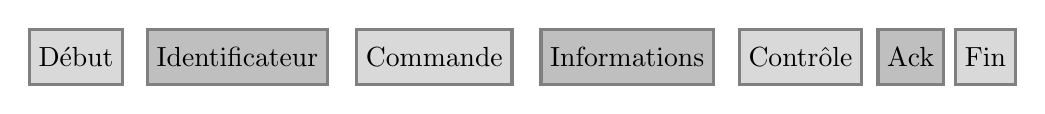
\begin{tikzpicture}[
block1/.style={rectangle, draw=black!50, fill=gray!30, very thick, minimum size=7mm},
block2/.style={rectangle, draw=black!50, fill=gray!50, very thick, minimum size=7mm},
]
%\shorthandoff{:} % Evite le bug de compilation avec tikz
    % Longueurs et espacement
    %\def\longabove{0.2cm}
    \def\espacement{2.35cm}

    % Définition des blocs
    \node [block1] (debut) {Début};
    \node [block2, right of=debut, node distance=2.05cm] (identificateur) {Identificateur};
    \node [block1, right of=identificateur, node distance=2.5cm] (com) {Commande};
    \node [block2, right of=com, node distance=2.45cm] (informations) {  Informations  };
    \node [block1, right of=informations, node distance=2.2cm] (controle) {Contrôle};
    \node [block2, right of=controle, node distance=1.4cm] (ack) {Ack};
    \node [block1, right of=ack, node distance=0.95cm] (fin) {Fin};
 
    % Définition des liens
%    \draw [<-] (codeur) -- ++(-2,0) node[left] {$\{b_n\}$};
%    \draw [->] (codeur) -- node[above=\longabove] {$\{d_n\}$} (cbs);
%    \draw [->] (cbs) -- node[above=\longabove] {$\{c_k\}$} (modulateur);
%    \draw [->] (modulateur) -- ++(2,0) node[right] {$s(t)$};
\end{tikzpicture}
